\documentclass[11pt,preprint]{elsarticle}

\usepackage{lmodern}
%%%% My spacing
\usepackage{setspace}
\setstretch{1.2}
\DeclareMathSizes{12}{14}{10}{10}

% Wrap around which gives all figures included the [H] command, or places it "here". This can be tedious to code in Rmarkdown.
\usepackage{float}
\let\origfigure\figure
\let\endorigfigure\endfigure
\renewenvironment{figure}[1][2] {
    \expandafter\origfigure\expandafter[H]
} {
    \endorigfigure
}

\let\origtable\table
\let\endorigtable\endtable
\renewenvironment{table}[1][2] {
    \expandafter\origtable\expandafter[H]
} {
    \endorigtable
}


\usepackage{ifxetex,ifluatex}
\usepackage{fixltx2e} % provides \textsubscript
\ifnum 0\ifxetex 1\fi\ifluatex 1\fi=0 % if pdftex
  \usepackage[T1]{fontenc}
  \usepackage[utf8]{inputenc}
\else % if luatex or xelatex
  \ifxetex
    \usepackage{mathspec}
    \usepackage{xltxtra,xunicode}
  \else
    \usepackage{fontspec}
  \fi
  \defaultfontfeatures{Mapping=tex-text,Scale=MatchLowercase}
  \newcommand{\euro}{€}
\fi

\usepackage{amssymb, amsmath, amsthm, amsfonts}

\def\bibsection{\section*{References}} %%% Make "References" appear before bibliography


\usepackage[numbers]{natbib}

\usepackage{longtable}
\usepackage[margin=2.3cm,bottom=2cm,top=2.5cm, includefoot]{geometry}
\usepackage{fancyhdr}
\usepackage[bottom, hang, flushmargin]{footmisc}
\usepackage{graphicx}
\numberwithin{equation}{section}
\numberwithin{figure}{section}
\numberwithin{table}{section}
\setlength{\parindent}{0cm}
\setlength{\parskip}{1.3ex plus 0.5ex minus 0.3ex}
\usepackage{textcomp}
\renewcommand{\headrulewidth}{0.2pt}
\renewcommand{\footrulewidth}{0.3pt}

\usepackage{array}
\newcolumntype{x}[1]{>{\centering\arraybackslash\hspace{0pt}}p{#1}}

%%%%  Remove the "preprint submitted to" part. Don't worry about this either, it just looks better without it:
\makeatletter
\def\ps@pprintTitle{%
  \let\@oddhead\@empty
  \let\@evenhead\@empty
  \let\@oddfoot\@empty
  \let\@evenfoot\@oddfoot
}
\makeatother

 \def\tightlist{} % This allows for subbullets!

\usepackage{hyperref}
\hypersetup{breaklinks=true,
            bookmarks=true,
            colorlinks=true,
            citecolor=blue,
            urlcolor=blue,
            linkcolor=blue,
            pdfborder={0 0 0}}


% The following packages allow huxtable to work:
\usepackage{siunitx}
\usepackage{multirow}
\usepackage{hhline}
\usepackage{calc}
\usepackage{tabularx}
\usepackage{booktabs}
\usepackage{caption}


\newenvironment{columns}[1][]{}{}

\newenvironment{column}[1]{\begin{minipage}{#1}\ignorespaces}{%
\end{minipage}
\ifhmode\unskip\fi
\aftergroup\useignorespacesandallpars}

\def\useignorespacesandallpars#1\ignorespaces\fi{%
#1\fi\ignorespacesandallpars}

\makeatletter
\def\ignorespacesandallpars{%
  \@ifnextchar\par
    {\expandafter\ignorespacesandallpars\@gobble}%
    {}%
}
\makeatother


% definitions for citeproc citations
\NewDocumentCommand\citeproctext{}{}
\NewDocumentCommand\citeproc{mm}{%
\href{\#cite.\detokenize{#1}}{#2}\nocite{#1}}

\makeatletter
% allow citations to break across lines
\let\@cite@ofmt\@firstofone
% avoid brackets around text for \cite:
\def\@biblabel#1{}
\def\@cite#1#2{{#1\if@tempswa , #2\fi}}
\makeatother
\newlength{\cslhangindent}
\setlength{\cslhangindent}{1.5em}
\newlength{\csllabelwidth}
\setlength{\csllabelwidth}{3em}
\newenvironment{CSLReferences}[2] % #1 hanging-indent, #2 entry-spacing
{\begin{list}{}{%
	\setlength{\itemindent}{0pt}
	\setlength{\leftmargin}{0pt}
	\setlength{\parsep}{0pt}
	% turn on hanging indent if param 1 is 1
	\ifodd #1
	\setlength{\leftmargin}{\cslhangindent}
	\setlength{\itemindent}{-1\cslhangindent}
	\fi
	% set entry spacing
	\setlength{\itemsep}{#2\baselineskip}}}
{\end{list}}

\usepackage{calc}
\newcommand{\CSLBlock}[1]{\hfill\break\parbox[t]{\linewidth}{\strut\ignorespaces#1\strut}}
\newcommand{\CSLLeftMargin}[1]{\parbox[t]{\csllabelwidth}{\strut#1\strut}}
\newcommand{\CSLRightInline}[1]{\parbox[t]{\linewidth - \csllabelwidth}{\strut#1\strut}}
\newcommand{\CSLIndent}[1]{\hspace{\cslhangindent}#1}


\urlstyle{same}  % don't use monospace font for urls
\setlength{\parindent}{0pt}
\setlength{\parskip}{6pt plus 2pt minus 1pt}
\setlength{\emergencystretch}{3em}  % prevent overfull lines
\setcounter{secnumdepth}{5}

%%% Use protect on footnotes to avoid problems with footnotes in titles
\let\rmarkdownfootnote\footnote%
\def\footnote{\protect\rmarkdownfootnote}
\IfFileExists{upquote.sty}{\usepackage{upquote}}{}

%%% Include extra packages specified by user

%%% Hard setting column skips for reports - this ensures greater consistency and control over the length settings in the document.
%% page layout
%% paragraphs
\setlength{\baselineskip}{12pt plus 0pt minus 0pt}
\setlength{\parskip}{12pt plus 0pt minus 0pt}
\setlength{\parindent}{0pt plus 0pt minus 0pt}
%% floats
\setlength{\floatsep}{12pt plus 0 pt minus 0pt}
\setlength{\textfloatsep}{20pt plus 0pt minus 0pt}
\setlength{\intextsep}{14pt plus 0pt minus 0pt}
\setlength{\dbltextfloatsep}{20pt plus 0pt minus 0pt}
\setlength{\dblfloatsep}{14pt plus 0pt minus 0pt}
%% maths
\setlength{\abovedisplayskip}{12pt plus 0pt minus 0pt}
\setlength{\belowdisplayskip}{12pt plus 0pt minus 0pt}
%% lists
\setlength{\topsep}{10pt plus 0pt minus 0pt}
\setlength{\partopsep}{3pt plus 0pt minus 0pt}
\setlength{\itemsep}{5pt plus 0pt minus 0pt}
\setlength{\labelsep}{8mm plus 0mm minus 0mm}
\setlength{\parsep}{\the\parskip}
\setlength{\listparindent}{\the\parindent}
%% verbatim
\setlength{\fboxsep}{5pt plus 0pt minus 0pt}



\begin{document}



\begin{frontmatter}  %

\title{Report Baby Names}

% Set to FALSE if wanting to remove title (for submission)




\author[Add1]{Tatjana Ebert}
\ead{}








\vspace{1cm}





\vspace{0.5cm}

\end{frontmatter}

\setcounter{footnote}{0}



%________________________
% Header and Footers
%%%%%%%%%%%%%%%%%%%%%%%%%%%%%%%%%
\pagestyle{fancy}
\chead{}
\rhead{}
\lfoot{}
\rfoot{\footnotesize Page \thepage}
\lhead{}
%\rfoot{\footnotesize Page \thepage } % "e.g. Page 2"
\cfoot{}

%\setlength\headheight{30pt}
%%%%%%%%%%%%%%%%%%%%%%%%%%%%%%%%%
%________________________

\headsep 35pt % So that header does not go over title




\section{Introduction}\label{introduction}

A New York based toy design agency requested an analysis of historical
baby naming trends in the United States between 1910 and 2014. The
objective is to determine whether popular names persist over time,
identify media-related naming spikes, and provide evidence-based
recommendations for selecting toy character names likely to remain
attractive to future consumers.

\subsection{Data Sources}\label{data-sources}

\begin{itemize}
\tightlist
\item
  US Baby Names by State (1910--2014)
\item
  Billboard Top 100 Charts
\item
  HBO Titles and Credits
\end{itemize}

\subsection{Objectives}\label{objectives}

\begin{itemize}
\tightlist
\item
  Measure persistence of popular names over time.
\item
  Identify major spikes in popularity.
\item
  Investigate media influences on naming behaviour.
\item
  Develop recommendations for toy character naming in the New York
  market.
\end{itemize}

\section{Persistence of Popular Baby
Names}\label{persistence-of-popular-baby-names}

\subsection{Spearman Rank Correlation
Analysis}\label{spearman-rank-correlation-analysis}

\begin{figure}[H]

{\centering 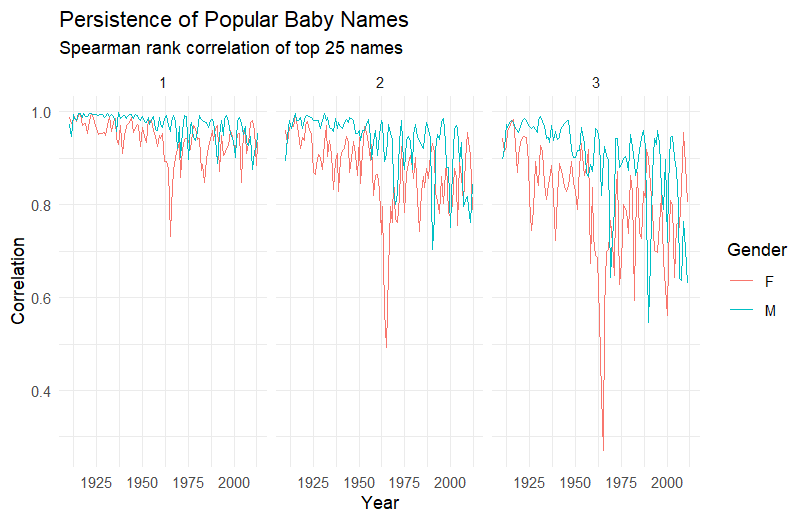
\includegraphics{../../graphs/Spearman} 

}

\caption{Persistence of popular baby names using Spearman rank correlations.}\label{fig:SpearmanPlot}
\end{figure}

\subsubsection{Key Findings}\label{key-findings}

\begin{itemize}
\tightlist
\item
  Popular names were highly persistent during most of the twentieth
  century.
\item
  Persistence declines as the comparison horizon increases from one to
  three years.
\item
  Naming persistence decreases noticeably after the 1990s.
\item
  Modern naming trends appear substantially more volatile.
\end{itemize}

\subsubsection{Interpretation}\label{interpretation}

Higher Spearman correlations indicate that the ranking of popular names
remains stable through time. Lower correlations imply that popular names
are replaced more rapidly by new trends.

\section{Before vs After 1990}\label{before-vs-after-1990}

\begin{figure}[H]

{\centering 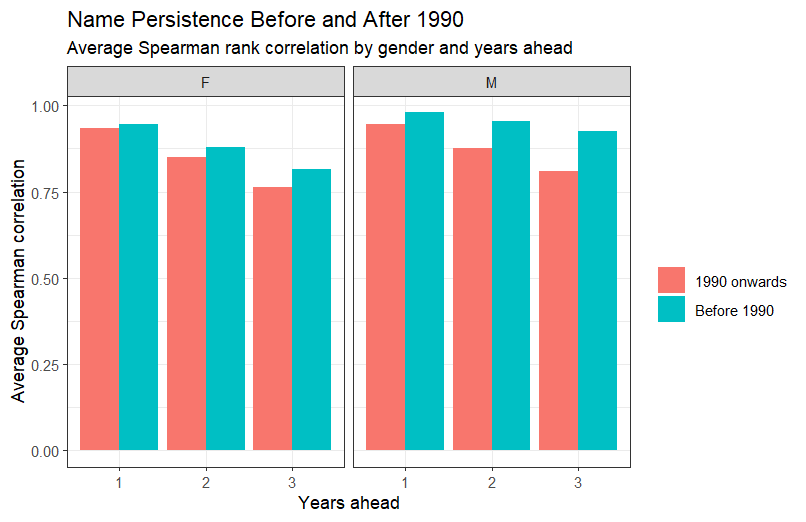
\includegraphics{../../graphs/Before_after_1900} 

}

\caption{Average name persistence before and after 1990.}\label{fig:BeforeAfter1990}
\end{figure}

\subsubsection{Key Findings}\label{key-findings-1}

\begin{itemize}
\tightlist
\item
  Average Spearman correlations are consistently higher before 1990.
\item
  Both boys' and girls' names exhibit reduced persistence after 1990.
\item
  The agency's hypothesis is supported.
\end{itemize}

\subsubsection{Business Implication}\label{business-implication}

\begin{itemize}
\tightlist
\item
  Modern naming trends change more rapidly.
\item
  Trend-driven toy names face a greater risk of becoming outdated.
\item
  Stable names are preferable for long-term product lines.
\end{itemize}

\section{Name Popularity Spikes}\label{name-popularity-spikes}

\subsection{Largest Relative Name
Spikes}\label{largest-relative-name-spikes}

\begin{figure}[H]

{\centering 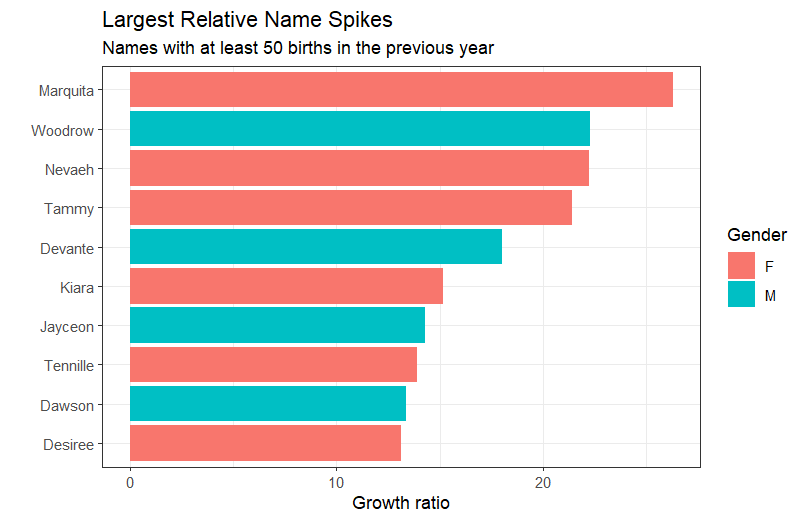
\includegraphics{../../graphs/relative_name_spikes} 

}

\caption{Largest relative increases in baby-name popularity.}\label{fig:RelativeSpikes}
\end{figure}

\subsubsection{Key Findings}\label{key-findings-2}

\begin{itemize}
\tightlist
\item
  Several names experienced explosive year-on-year growth.
\item
  Relative spikes typically occur among previously uncommon names.
\item
  Many spikes appear linked to cultural and media influences.
\end{itemize}

\subsection{Largest Absolute Name
Spikes}\label{largest-absolute-name-spikes}

\begin{figure}[H]

{\centering 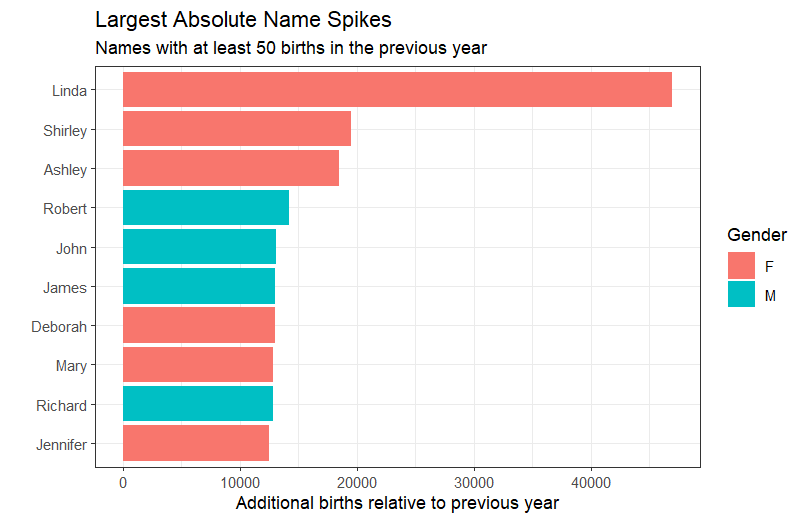
\includegraphics{../../graphs/absolute_name_spikes} 

}

\caption{Largest absolute increases in baby-name popularity.}\label{fig:AbsoluteSpikes}
\end{figure}

\subsubsection{Key Findings}\label{key-findings-3}

\begin{itemize}
\tightlist
\item
  Absolute spikes identify names that achieved widespread adoption.
\item
  These names reflect broad national popularity rather than niche
  trends.
\item
  Large absolute increases often indicate substantial cultural
  influence.
\end{itemize}

\section{Media Influence on Naming}\label{media-influence-on-naming}

\subsection{Case Study: Whitney}\label{case-study-whitney}

\begin{figure}[H]

{\centering 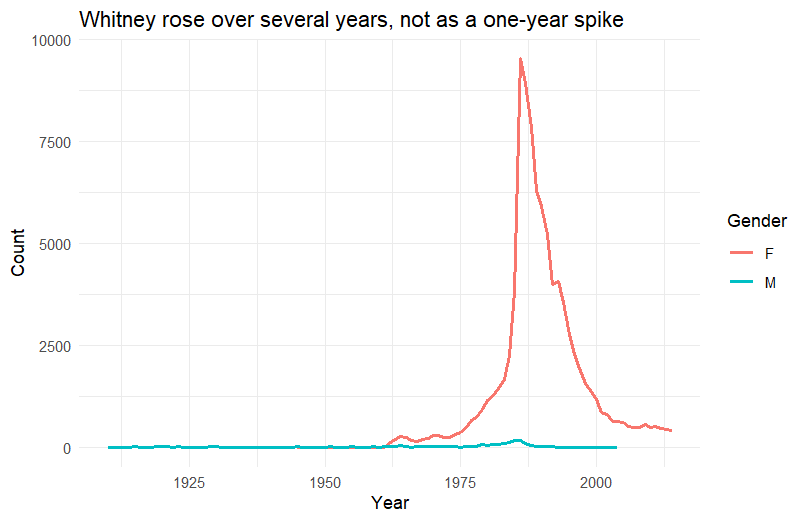
\includegraphics{../../graphs/Whitney} 

}

\caption{Popularity of the name Whitney through time.}\label{fig:WhitneyPlot}
\end{figure}

\subsubsection{Key Findings}\label{key-findings-4}

\begin{itemize}
\tightlist
\item
  Whitney displays sustained growth during the 1980s.
\item
  The increase coincides with the popularity of Whitney Houston.
\item
  The pattern reflects long-term cultural influence rather than a
  one-year fad.
\end{itemize}

\subsubsection{Business Implication}\label{business-implication-1}

\begin{itemize}
\tightlist
\item
  Celebrity-associated names can generate lasting public recognition.
\item
  Names with enduring cultural relevance may provide stronger branding
  opportunities.
\end{itemize}

\section{Long-Term Naming Trends}\label{long-term-naming-trends}

\subsection{Evolution of Selected
Names}\label{evolution-of-selected-names}

\begin{figure}[H]

{\centering 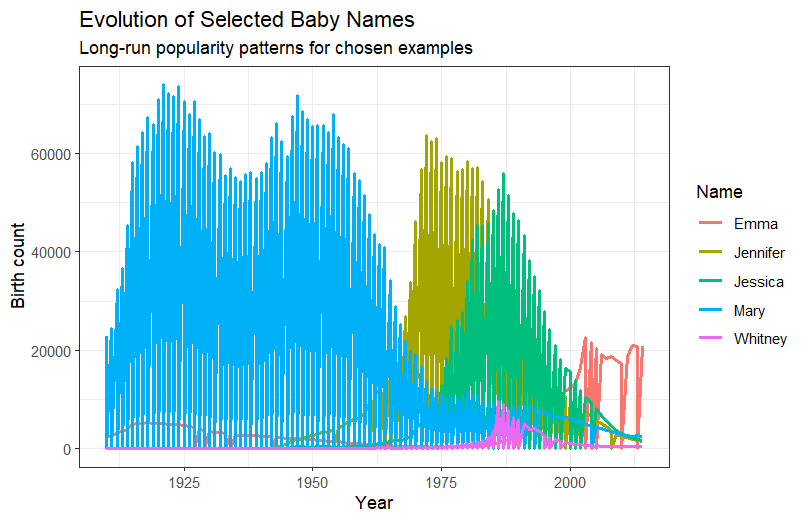
\includegraphics{../../graphs/Selected_names_evolution} 

}

\caption{Evolution of selected baby names through time.}\label{fig:SelectedNames}
\end{figure}

\subsubsection{Key Findings}\label{key-findings-5}

\begin{itemize}
\tightlist
\item
  Some names remain popular across multiple generations.
\item
  Others exhibit distinct rise-and-fall cycles.
\item
  Naming preferences evolve considerably through time.
\end{itemize}

\subsection{Top Names by Decade}\label{top-names-by-decade}

\begin{figure}[H]

{\centering 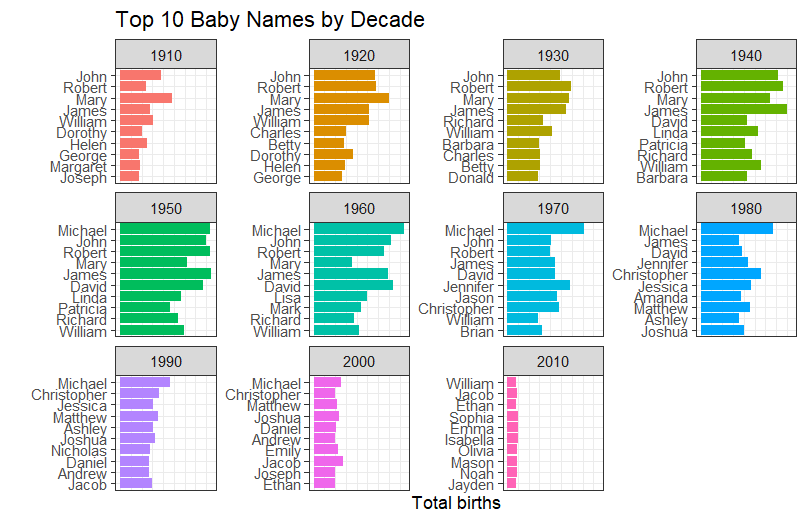
\includegraphics{../../graphs/Top_names_by_decade} 

}

\caption{Top baby names by decade.}\label{fig:TopNamesByDecade}
\end{figure}

\subsubsection{Key Findings}\label{key-findings-6}

\begin{itemize}
\tightlist
\item
  Distinct naming fashions emerge in different decades.
\item
  Some names dominate only a single generation.
\item
  Other names demonstrate remarkable longevity.
\end{itemize}

\subsection{Decade Heatmap}\label{decade-heatmap}

\begin{figure}[H]

{\centering 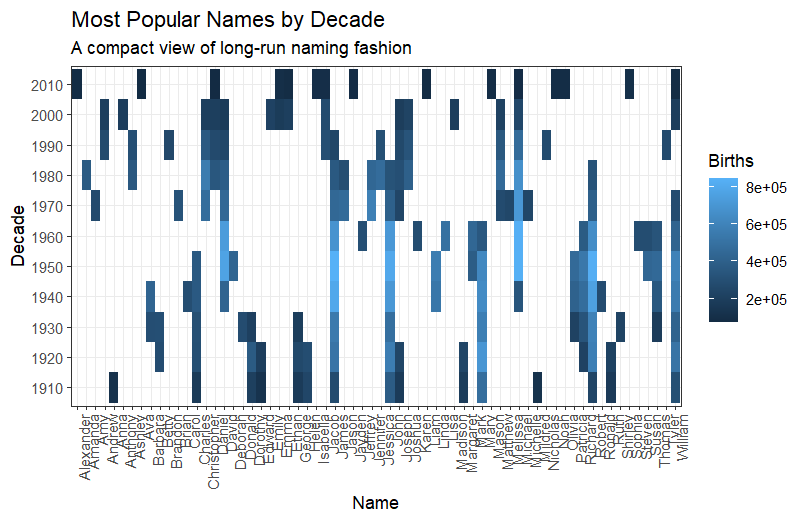
\includegraphics{../../graphs/Decade_heatmap} 

}

\caption{Heatmap of the most popular names by decade.}\label{fig:DecadeHeatmap}
\end{figure}

\subsubsection{Key Findings}\label{key-findings-7}

\begin{itemize}
\tightlist
\item
  The heatmap highlights changing naming fashions over time.
\item
  Long-lived names remain visible across multiple decades.
\item
  Most names experience finite popularity cycles.
\end{itemize}

\section{New York Toy Character Name
Analysis}\label{new-york-toy-character-name-analysis}

\subsection{Recommended Toy Names}\label{recommended-toy-names}

A toy-name score was developed using popularity, longevity and stability
within New York State.

\begin{figure}[H]

{\centering 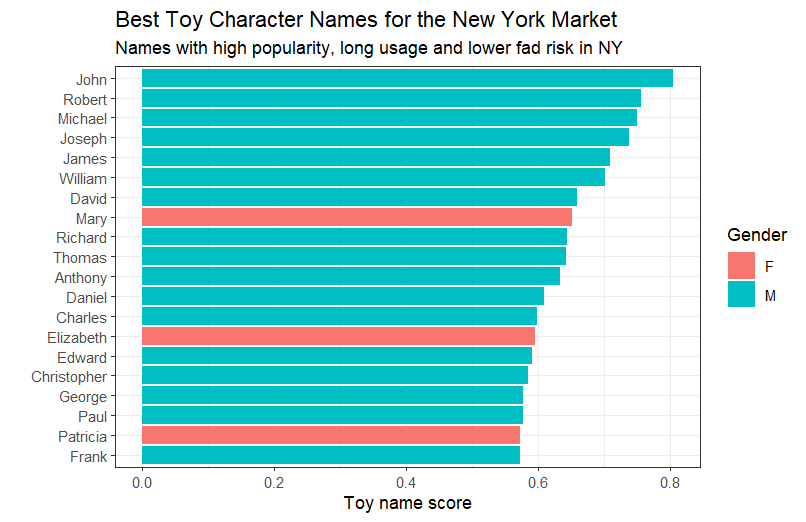
\includegraphics{../../graphs/best_toy_names_ny} 

}

\caption{Highest scoring toy character names in New York.}\label{fig:BestToyNamesNY}
\end{figure}

\subsubsection{Key Findings}\label{key-findings-8}

\begin{itemize}
\tightlist
\item
  Recommended names combine popularity and long-term stability.
\item
  These names are familiar to multiple generations of consumers.
\item
  Such names represent lower branding risk.
\end{itemize}

\subsection{High-Risk Toy Names}\label{high-risk-toy-names}

\begin{figure}[H]

{\centering 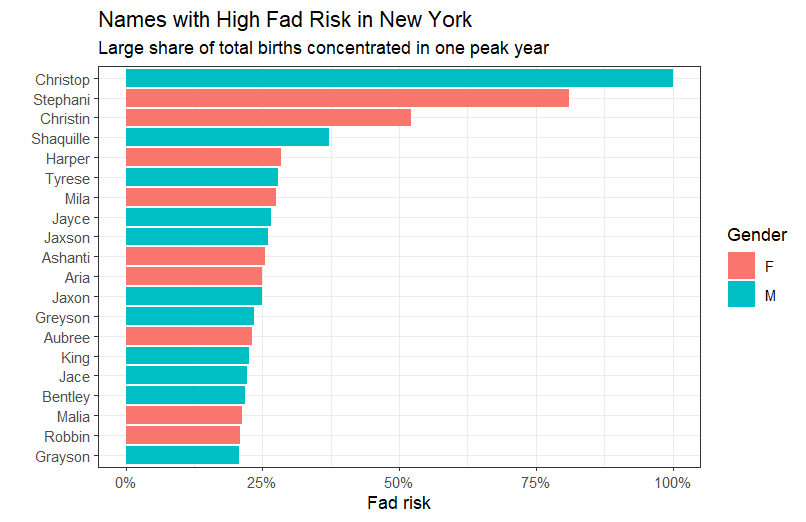
\includegraphics{../../graphs/risky_toy_names_ny} 

}

\caption{Names exhibiting high fad risk in New York.}\label{fig:RiskyToyNamesNY}
\end{figure}

\subsubsection{Key Findings}\label{key-findings-9}

\begin{itemize}
\tightlist
\item
  These names concentrate popularity within a short period.
\item
  They are more vulnerable to changing trends.
\item
  Such names may be suitable for short-term products but not flagship
  brands.
\end{itemize}

\section{Recommendations}\label{recommendations}

\subsection{Long-Term Toy Franchises}\label{long-term-toy-franchises}

Recommended characteristics:

\begin{itemize}
\tightlist
\item
  High persistence
\item
  High popularity
\item
  Low volatility
\item
  Multi-generational familiarity
\end{itemize}

Benefits:

\begin{itemize}
\tightlist
\item
  Lower branding risk
\item
  Greater longevity
\item
  Broader market appeal
\end{itemize}

\subsection{Trend-Based Product Lines}\label{trend-based-product-lines}

Recommended characteristics:

\begin{itemize}
\tightlist
\item
  Strong recent growth
\item
  Association with celebrities, music or television
\end{itemize}

Benefits:

\begin{itemize}
\tightlist
\item
  Immediate recognition
\item
  Potential short-term sales boost
\end{itemize}

Risks:

\begin{itemize}
\tightlist
\item
  Higher probability of becoming outdated
\end{itemize}

\section{Conclusion}\label{conclusion}

Analysis of US baby naming trends indicates that naming persistence has
declined since approximately 1990, resulting in shorter-lived naming
fashions. Media and celebrity influences continue to shape naming
behaviour and can generate substantial popularity increases. For a New
York toy design agency, names demonstrating long-term stability and
broad familiarity provide the strongest foundation for sustainable toy
branding, while highly volatile names are better suited to short-term
marketing opportunities.

\bibliography{Tex/ref}





\end{document}
